In this section, we provide
our approach to solving the 
schedule learning problem. 
We assume that a TPN
is learned from event data using
existing approaches, e.g., via the approach presented 
in~\cite{DBLP:conf/bpm/SenderovichRGMM15}.
\todo{we actually make a modification that enables 
	that some of the activities can be performed by alternating sets of resources}.

\subsection{Seize-Delay-Release Nets}

The transformation of a learned TPN into a BSP,
is based on the notion 
of Seize-Delay-Release nets with resources (SDRR nets). 

To define SDRR nets, 
we first consider seize-delay-release constructs (SDCs), 
which are 
TPNs that consist of the following three components:
(1) two transitions: one immediate transition that seizes a token and 
one timed transition that releases the token after a delay, (2) a place where the
token is delayed, and (3) two flows that connect the two transitions to the delay place. 
Formally,
\begin{mydef} [Seize-Delay Construct (SDC)] \label{def:sdc}
	An SDC is a timed Petri net, 
	$\mathcal{S} = \langle E, E' , P , F, \tau \rangle)\rangle$, such that 
	\begin{itemize}
		\item The set $E = \{ e_{seize}, e_{release} \}$ contains two transitions (seize and delay), 
		\item The set $E' = \{e_{release}\}$ is the timed delay transition, 
		\item The set $P = \{p_{delay}\}$ is a single delay place, and,
		\item The flow is $F = \{ (e_{seize}, p_{delay}), (p_{delay}, e_{release})\}$.
	\end{itemize}
\end{mydef} The gray parts in Figure~\ref{fig:sdr-net} are the three 
SDC components of the TPN.
The SDC that directly follows the start place in Figure~\ref{fig:sdr-net} contains an immediate
transition, which seizes the token in the start place. 
Then, the token is delayed for $\tau(e_{release})$,
which corresponds to the duration of the `Exam'
transition. Lastly, `Exam' releases the token into the subsequent place.

\begin{figure}[t!]
	\centering
	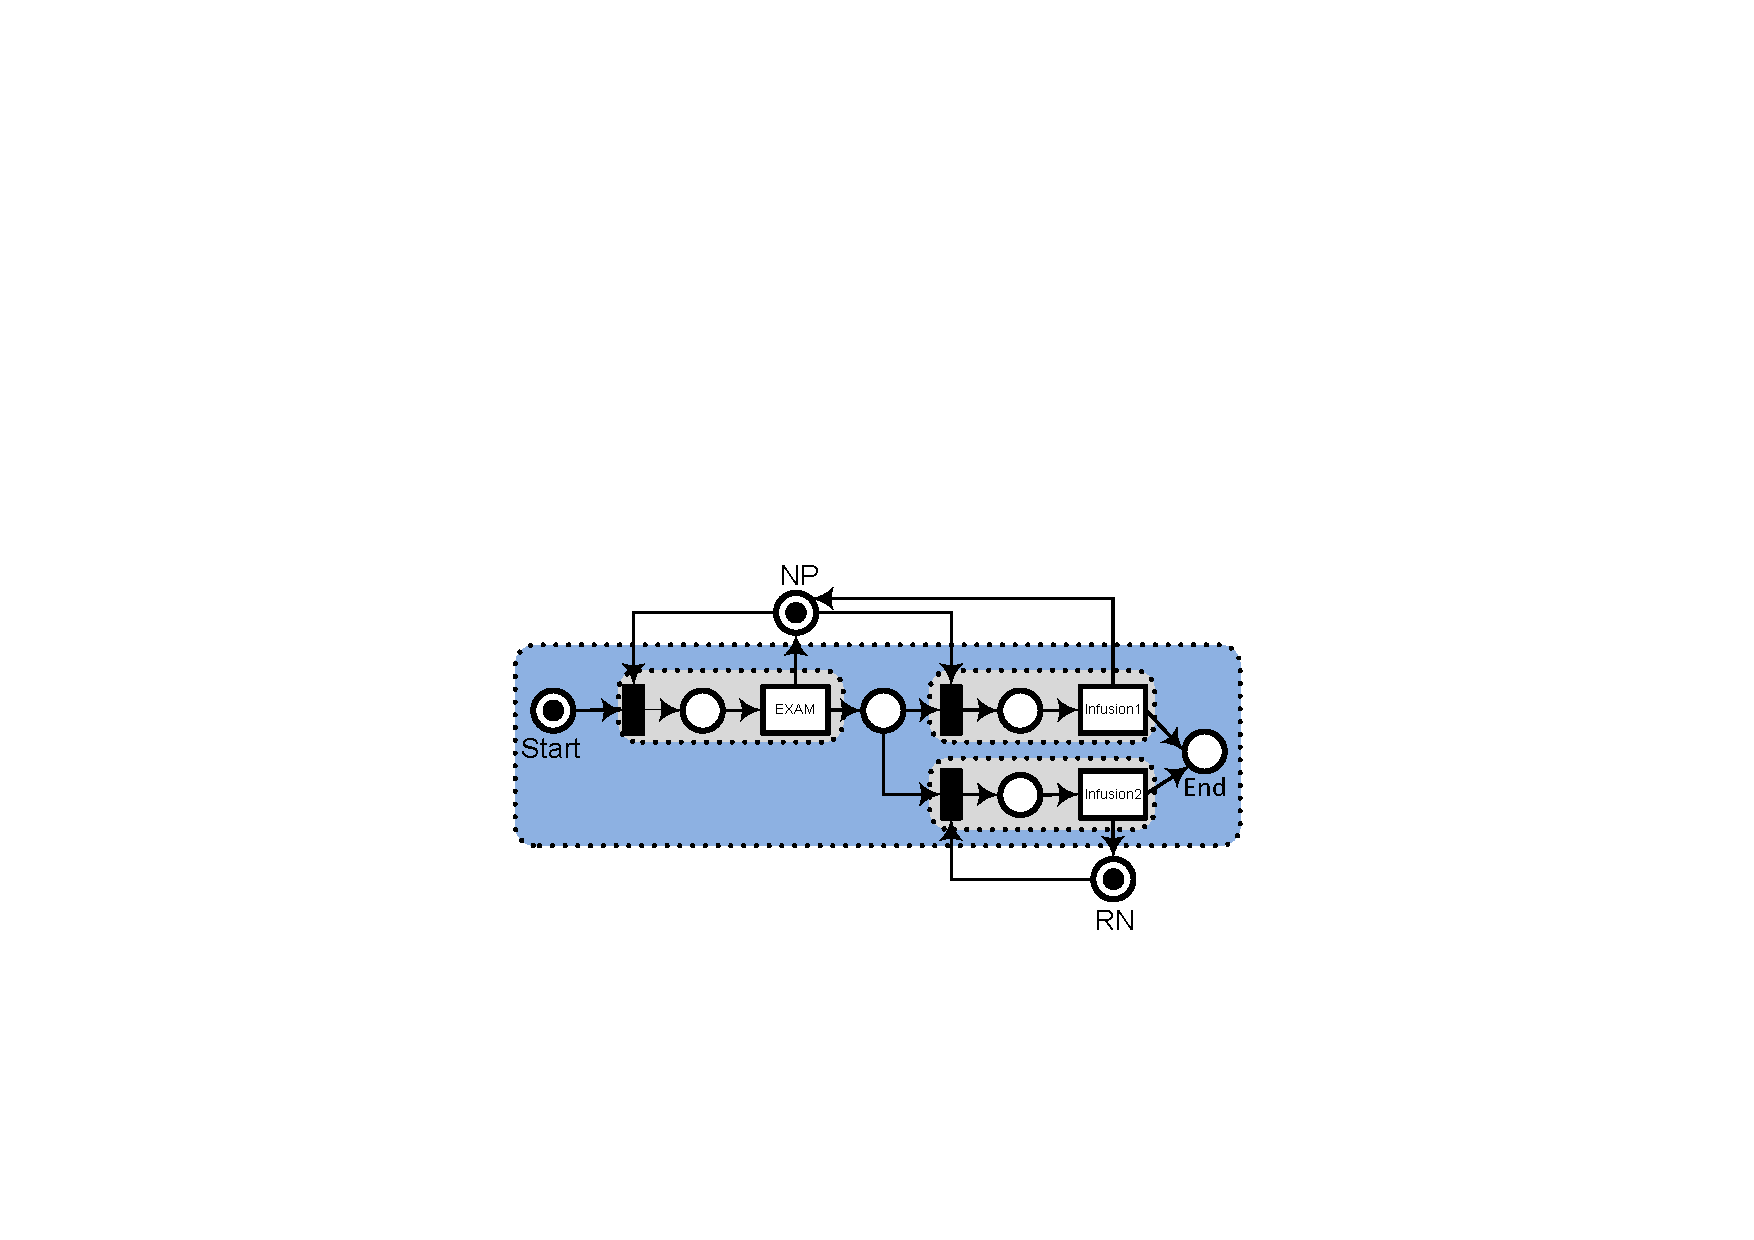
\includegraphics[scale=0.6]{SDNet.pdf}
	\caption{An SDRR Net of a Hospital Process.}
	\label{fig:sdr-net}  
	\vspace{-1em}
\end{figure}



Given an SDC, $\mathcal{S}$, we denote
$E_{\mathcal{S}}$ (and $E_{\mathcal{S}}'$), $P_{\mathcal{S}}$, $F_{\mathcal{S}}$ its
sets of transitions (and timed transitions), places and flows,  respectively.
Furthermore, the set of places that precede (follow) the immediate (timed) transition of $\mathcal{S}$ is denoted by 
$\bullet E_{\mathcal{S}}$ ($E_{\mathcal{S}} \bullet$), i.e., \begin{align*}
&\bullet E_{\mathcal{S}} = \{p \in P \ | \ \forall e \in E_{\mathcal{S}} \setminus E_{\mathcal{S}}': \ p \in \bullet e \} \\
&E_{\mathcal{S}} \bullet = \{p \in P \ | \ \forall e' \in E_{\mathcal{S}}' : \ p \in e'\bullet \}. \\
\end{align*}

Detecting the SDCs of a given TPN is linear in the number of transitions ($\mathcal{O}(|E|+|P|)$), since 
it involves traversing over the immediate transitions of the TPN and verifying
that the transition is followed by a single place,
which is in turn followed by 
a single timed transition (see Definition~\ref{def:sdc}).



A TPN that comprises a set of SDCs is referred to 
as a seize-delay-release net (SDR net). To define 
an SDR net, we let $S= \{\mathcal{S}_1,\ldots,\mathcal{S}_m\}$ be a set of SDCs.
The set $S$ can be partitioned into 
$k$ sets denoted by $C = \{\mathcal{C}_1,\ldots, \mathcal{C}_k\}$, 
with each set $\mathcal{C}_j, j = 1,\ldots, k$ containing 
SDCs that have equal 
input and output places. It is easy to show 
that $C$ always exists and that it is unique for 
a given TPN.
To simplify notation, we denote $E_{\mathcal{C}_j}$ ($E_{\mathcal{C}_j}'$)
the transitions (timed transitions)
of the SDCs that are elements of 
$\mathcal{C}_j$. We are now ready to define 
seize-delay-release nets.

\begin{mydef} [Seize-Delay-Release Net] \label{def:sdnet}
	A seize-delay-release net is a timed Petri net, 
	$\mathcal{N}_{sdr} = (E, E', P , F, \tau)$, which satisfies the following
	conditions:
	\begin{itemize}
		\item The set $\bigcup_{j=1}^{m} E_{\mathcal{S}_j}$ contains only transitions 
		from the set of SDCs ($E' \subseteq E$ being 
		the set of timed transitions), 
		\item The set $P = \bigcup_{j=1}^m P_{\mathcal{S}_j} \cup P_{c}$ contains 
		both the delay places
		of $N$ and a finite set of $k+1$ connector places $P_{c} = \{p_1,\ldots, p_{k+1}\}$
		with $p_1, p_{k+1} \in P_c$ being unique source and sink places, respectively, and, 
		\item The flow $F = \bigcup_{j=1}^m F_{\mathcal{S}_j} \cup F_c$ contains
		both the set of SDC
		flows and a set $F_c$ 
		such that \begin{align} \label{eq1}
		F_c = & \{(p,e) \in P_c \times E \setminus E' \ | \\ & p = p_j \ \land \exists\mathcal{C}_j \in C (\ e \in E_{\mathcal{C}_j} \setminus E_{\mathcal{C}_j}') \} \ \cup \nonumber\\
		&\{(e,p) \in E' \times P_c \ | \\ &\exists \mathcal{C}_j \in C (e \in E_{\mathcal{C}_j}' \ \land \ p = p_{j+1}) \}.
		\end{align}
	\end{itemize}
\end{mydef} An example for an SDR net can be found in Figure~\ref{fig:sdr-net}. The blue area corresponds to an SDR net that consists of three SDCs partitioned
into two sets, namely an SDC that involves `Exam' and two SDCs that correspond to Infusion 
(transitions Infusion1 and Infusion2 are 
part of the same set in the partition of SDCs, $C$). Furthermore,
the place of connectors $P_c$ contains three places: start place, 
end place and 
a place that connects `Exam' to the two `Infusion' SDCs.
SDR nets are important building blocks of the
Seize-Delay-Release nets with resources (SDRR nets),
which we map into basic scheduling problems. Algorithm~\ref{Alg1} verifies that a TPN
is an SDR net.



\begin{algorithm}[h!]
	
	\LinesNumbered
	\DontPrintSemicolon
	\SetAlgoLined
	\KwIn{Timed Petri net $\mathcal{N} = \langle E, E',P, F, \tau \rangle$}
	\KwOut{$\langle \{\mathcal{S}_1,\ldots,\mathcal{S}_m\}, P_c \rangle$ - Set of SDCs and set
		of connector places $P_c$}
	\Begin{
		
		
		$P_{in} \leftarrow \{p \in P \ | \ \bullet p = \emptyset\}$\;
		$P_{out} \leftarrow \{p \in P \ | \ p \bullet = \emptyset\}$\;
		\uIf{$|P_{in}| \neq 1 \ \lor |P_{out}| \neq 1 $}
		{\Return False \; }
		
		$S = \{\mathcal{S}_1,\ldots,\mathcal{S}_m\} \leftarrow$ \emph{DetectSDC}$(\mathcal{N})$\;
		
		\uIf{$\bigcup_{j=1}^{m} E_{\mathcal{S}_j} \neq E$}
		{\Return False \; }
		
		$C \leftarrow \{\mathcal{C} \subseteq S \ | \ \forall \mathcal{S}_i,\mathcal{S}_j \in \mathcal{C} :$ \ $ \bullet E_{\mathcal{S}_i} = \bullet E_{\mathcal{S}_j} \ \land \
		E_{\mathcal{S}_i} \bullet =  E_{\mathcal{S}_j} \bullet\}$\;
		
		
	
		\ForEach{$\mathcal{C}_j \in C$}{
		$\bullet\mathcal{C}_j = \bigcup_{\mathcal{S} \in \mathcal{C}_j} \bullet E_{\mathcal{S}}$\;
		$\mathcal{C}_j\bullet = \bigcup_{\mathcal{S} \in \mathcal{C}_j} E_{\mathcal{S}} \bullet$\;
		\uIf{$(\bullet\mathcal{C}_j =  \mathcal{C}_j\bullet \ \lor \ 
			|\bullet\mathcal{C}_j| \neq 1 \ \lor 
			\ |\mathcal{C}_j\bullet| \neq 1$}{\Return False \;}	
		
		}
		\uIf{$\exists \mathcal{C}_i \neq \mathcal{C}_j \in C \ (\mathcal{C}_i \bullet = \mathcal{C}_j \bullet 
		\ \lor \ \bullet\mathcal{C}_i  = \bullet\mathcal{C}_j)) $}{\Return False \;}	
	
		
		$P_c \leftarrow \bigcup_{\mathcal{C}_j \in C} (\bullet\mathcal{C}_j \cup  \mathcal{C}_j \bullet) $\;
		$F_c \leftarrow \bigcup_{\mathcal{C}_j \in C} \{(x,y) \in F \ | \  (x \in \bullet\mathcal{C}_j \ \land \ y \in E_{\mathcal{C}_j} \setminus E_{\mathcal{C}_j}' ) \ \lor \ (x \in E_{\mathcal{C}_j}' \ \land \ y \in \mathcal{C}_i \bullet)\}$\;

		
		\uIf{$P_c \neq P \setminus \bigcup_{j=1}^{m} P_{\mathcal{S}_j} \ \lor \ F_c \neq F \setminus \bigcup_{j=1}^{m} F_{\mathcal{S}_j}$}
		{\Return False \; }
		\Return True \;
	}
	
	
	\caption{Verifies that TPN is SDR net.}
	\label{Alg1}
\end{algorithm}

\todo{update explanation and proof}
  


Below, we explain the algorithm line-by-line. Lines 2-5
verify that the TPN has unique input and output places. Line 6 
returns the set of SDCs, $S$, that 
are present in 
the input TPN. 
Detecting SDCs is performed via the function \emph{DetectSDC}$(\cdot)$,
which uses a simple traversal over all immediate transitions 
$e \in E \setminus E'$ and checking whether the direct followers of $e$ are 
a single place and a timed transition (as in Definition~\ref{def:sdc}). 
Lines 7-8 make sure that the set of transitions $E$ includes
only transitions from $S$. 

Line 9 partitions 
the SDCs into sets of SDCs, such that
each set $\mathcal{C} \in C$ contains only 
SDCs that share input and output places. 

Lines 10-15 traverse the sets in $C$ and 
verify that each set $\mathcal{C}_j \in C$ has a unique input 
place and a unique output place 
($|\bullet\mathcal{C}_j| = |\mathcal{C}_j\bullet| =1$). 
Furthermore, Lines 10-13
ensure that the input and output places of $\mathcal{C}_j$
are not equal to each other (no loops), and that 
there does not exist an additional set $\mathcal{C}_i \neq \mathcal{C}_j$
for which one of its input or output places are equal to 
the corresponding input and output places of $\mathcal{C}_j$. 
Intuitively, this enforces a sequential execution of the sets 
of SDCs in $C$. Lines 14-17 check whether the TPN places
can be either SDC places or connectors ($P_c$)
and that the only flows allowed in the TPN 
are within SDCs or between connector places, $P_c$, 
and SDC constructs.

If the algorithm reaches Line 18 without breaking,
it concludes that the TPN is an SDR net and returns its set of SDCs $S$ and
the set of connector places $P_c$. Proposition~\ref{prop:corrAlg1} states the 
correctness and completeness of Algorithm~\ref{Alg1}.
\todo{polish proof}

\begin{myprop} \label{prop:corrAlg1}
	Algorithm~\ref{Alg1} is correct and complete, 
	i.e., the algorithm returns non-empty sets, if and only if, the input TPN
	is an SDR net. 
\end{myprop}
\begin{proof} \noindent \emph{If: Given an input TPN that is an SDR net, the algorithm returns non-empty sets.}\\
	The input TPN is an SDR net. Hence, by Definition~\ref{def:sdnet}, it has a source and a sink. Furthermore, $E = \bigcup_{j=1}^m E_{\mathcal{S}_j}$
	and therefore Lines 4 and 7 return True. 
	In an SDR net, all flows are either 
	in $\bigcup_{j=1}^m F_{\mathcal{S}_j}$ (being part of an SDC) 
	or in $F_c$, i.e., connecting places in $P_c = \{p_1,\ldots, p_{k+1}\}$
	to the set of SDCs in the partition set, $C$. Furthermore, from the definition of $F_c$ 
	each partition set $\mathcal{C}_j$ has exactly a single direct predecessor place $p_j \in P_c$
	and a single direct successor place $p_{j+1}$. Moreover, no two 
	sets in $C$ can have the exact same predecessors and successors (otherwise, they would 
	not be two different sets in $C$). Therefore, the condition in Line 13
	holds for every $\mathcal{C}_j \in C$.\\	
		
	\noindent \emph{and only If: 
	Given that the algorithm returns non-empty sets, the input net is an SDR net.}\\
	We prove the second direction by using the intermediate 
	computations
	of Algorithm~\ref{Alg1} to construct an SDR net $\mathcal{N} = (E, E',P, F, \tau)$
	and showing that the net $\mathcal{N}$ is equal to the input TPN. 
	
	
		

	
\end{proof}


Having defined SDR nets and an algorithm that verifies whether 
a given TPN is an SDR net, we
define the seize-delay-release net with resources (SDRR net),
which is a timed Petri net that consists of a set of SDR nets and a set of places
and flows that correspond to resources. Let $N_{sdr} = \{\mathcal{N}_1,\ldots,\mathcal{N}_n\}$ be a set of 
SDR nets with $\mathcal{N}_j = \langle E_j, E'_j , P_j , F_j, \tau_j\rangle, j = 1, \ldots, n$ and
let $S = \{\mathcal{S}_1,\ldots,\mathcal{S}_m\}$ be a set of SD constructs
that participate in $N_{sdr}$. We are now ready to define the SDRR nets. 

\begin{mydef} [Seize-Delay-Release Net with Resources (SDRR net)] \label{def:sdr-net}
	An SDR net with resources (SDRR net) is a timed Petri net, 
	$\mathcal{N}_{sdrr} = (E, E', P , F, \tau)$, such that 
	\begin{itemize}
		\item The set \small $E = \bigcup_{j=1}^n E_j$ contains only transitions from the SDNs ($E' \subseteq E$ being 
		the set of timed transitions), 
		\item The set \small $P = \bigcup_{j=1}^m P_j \cup P_{r}$ contains both places from $N$ 
		and a finite set of resource places $P_{r}$, and, 
		\item The flow set \small $F = \bigcup_{i=1}^m F_i \cup F_r$ contains		
		all SDN 
		flows and a set $F_r$ 
		such that:  
		\small
		\begin{align*}
		F_r = &\{ (x,y) \in (P_r \times E \setminus E') \cup
		(E' \times P_r) \ | \ \forall (x,y) \in F_r: \\  &Q(x,y,S) \}
		\end{align*}
		with, \small \begin{align*} &Q(x,y,S) =\\ 
		&((x \in P_r \land y \in E_{\mathcal{S}_i} \setminus E_{\mathcal{S}_i}'  \Rightarrow \exists (e',x) \in F_r: \ e' \in E_{\mathcal{S}_i}') \\
		& \land \ (x \in E_{\mathcal{S}_i}' \land y \in P_r \Rightarrow \exists (y,e) \in F_r: \ e \in E_{\mathcal{S}_i} \setminus E_{\mathcal{S}_i}').\end{align*}
	\end{itemize}
\end{mydef} The set of resource flows $F_r$ allows for resource tokens to be consumed only by immediate transitions and produced 
only by timed transitions. Furthermore, the property $Q(x,y)$ makes sure that 
if an immediate 
transition that consumes a resource token 
is part of an SDC, say $\mathcal{S}_i$, then there must 
also be a flow between the timed transition of $\mathcal{S}_i$ back
to the same resource place. Similarly, if a timed transition of an SDC produces a resource 
token, there must be a flow between the resource 
place and the immediate transition of the same SDC.
One
can easily verify that Figure~\ref{fig:sdr-net} 
is an SDRR net with a single SDR net, three SDCs and two resource places 
($NP$ for nurse practitioner and $RN$ for registered nurse). 


Next, we introduce Algorithm~\ref{Alg2},
which  
take a TPN as its input, and returns
whether the TPN is an SDRR net. 


\begin{algorithm}[h!]
	
	\LinesNumbered
	\DontPrintSemicolon
	\SetAlgoLined
	\KwIn{Timed Petri net $\mathcal{N} = \langle E, E',P, F, \tau \rangle$}
	\KwOut{True or False}
	\Begin{
		
		%\tcc{Step 1: Find resource places by removing}
		$S = \{\mathcal{S}_1,\ldots,\mathcal{S}_m\} \leftarrow$ \emph{DetectSDC}$(\mathcal{N})$\;
		$P_r \leftarrow \{p \in P \ | \ \forall (x,y) \in F_{\{p\}} ( Q(x,y,S))  \}$\;
		$\mathcal{N}' =(E, E',P \setminus P_r, F \setminus F_{P_r}, \tau)$\; 
		$\{\mathcal{N}_i\}_{i=1}^{n} \leftarrow$ \emph{ConnectedComponents}$(\mathcal{N}')$\;
		\uIf{$\exists i \in [n] :$ \emph{VerifySDR}$(\mathcal{N}_i) $ = False}
		{\Return False\;}

		\Return True\;
	}


	\caption{Verifies that TPN is SDR net with resources (SDRR net).}
	\label{Alg2}
\end{algorithm}

\todo{update this part for the new algorithm}
We shall briefly go over the algorithm and 
explain its parts. Lines 2-7 serve us to identify 
a set of places $P_r$ that are candidates to be
the resource places of the resulting SDRR. 
In an SDRR,
a necessary condition for every $p \in P_r$ is 
that when $p$ is removed from the net (along
with the incoming and outgoing flows $F_{\{p\}}$) 
there will still exist a path between SDR net sources 
to their corresponding sinks. Removing a non-resource place,
i.e., a place from one of the SDR nets of the SDRR net, 
will result in a source without a path to its sink. 
Therefore, removing places from the input TPN
and verifying that every source has a path to a sink (via the
function \emph{AllSourceToSink} that receives a TPN and checks whether 
every source has a path to a sink),
enables us to find candidates for $P_r$. 
Then, in Line 8, we remove all places in $P_r$ from the input TPN
and store the resulting net $\mathcal{N}'$. In Line 9,
we store the connected components of $\mathcal{N}'$ in a set of
TPNs $\{\mathcal{N}_i\}_{i=1}^{n}$. If the input is an SDRR, 
this set will contain $n$ SDR nets. Therefore, in Lines 12-18,
we verify that the $n$ connected components are SDR nets. 
Verifying whether $\mathcal{N}_i$ is an SDR net 
is performed by running a 
Breadth-First Search (BFS) algorithm that 
verifies the conditions in Definition~\ref{def:sdnet}.
The procedure \emph{VerifySDR}$(\cdot)$ returns $\emptyset$
if $\mathcal{N}_i$ is not an SDR (which will lead to 
an answer False in Algorithm~\ref{Alg2} due to a violation of Definition~\ref{def:sdr-net});
otherwise,
it returns the set $P_{c,i}$, which is the connector set of the
now verified SDR net $\mathcal{N}_i$, and $S_i$,
which is the set of SDCs that $\mathcal{N}_i$ comprises.
Lastly, Lines 19-20 check whether the set of 
candidate resource places, $P_r$, satisfies $Q(x,y,S)$ 
from Definition~\ref{def:sdr-net}. If one of the flows
into $p \in P_r$ violates $Q(x,y,S)$, the algorithm returns False.
Otherwise, the algorithm returns True.


 \todo{polish proof}
\begin{myprop} \label{prop:corrAlg2}
	Algorithm~\ref{Alg2} is correct and complete, 
	i.e., the algorithm returns \emph{True}, if and only if, the input to the algorithm
	is an SDRR net. 
\end{myprop}
\begin{proof} \noindent \emph{If: Given an input TPN that is an SDRR net, the algorithm returns True.}\\
If $\mathcal{N}$ is an SDRR net, then the only places that would not interrupt the flow between every source 
and sink of its SDR nets in $N_{sdr}$, are places in $P_r$. 
Therefore, the set $P_r$ computed by the algorithm will contain only resource places
of the SDRR net. 
After removing the resource places and their corresponding flows (Line 8),
we are remained with $n$ connected components, with each component being an SDR net (Line 9).
The algorithm will verify the following two conditions: (1) the $n$ components are SDR nets (Lines 10-18),
and (2) the set of flows $F_r$ respects $Q(x,y,S)$ (since the TPN is an SDRR net). Therefore it will return 
True.\\

	
	
\noindent \emph{and only If: Given that the algorithm returns True, the input net is an SDRR net.}\\
We prove the second direction by using the intermediate 
computations
of Algorithm~\ref{Alg1} to construct a Petri net $\mathcal{N} = (E, E',P, F, \tau)$
and showing that $\mathcal{N}$ corresponds to an SDRR net (Definition~\ref{def:sdr-net}). We
compose the SDRR net by 
connecting the TPNs $\mathcal{N}_i, i = 1, \ldots, n$ (which are verified to be SDR nets by Lines 10-18) to the set of places
$P_r$ using the flow set $F_r$. Since the flows $F_r$ respect property $Q(x,y)$, 
the resulting net is an SDRR net according to Definition~\ref{def:sdr-net}.

\end{proof}


